%\documentclass{vldb}
\documentclass[10pt,conference,letterpaper]{IEEEtran}

\usepackage{times}
\usepackage{graphicx}
\usepackage{listings}
\usepackage{color}
\usepackage{url}
\usepackage{amsmath}


\sloppy

\newcommand{\marcos}[1]{\ \\ \fbox{\parbox{1.0\linewidth}{{\sc Marcos}:\\ #1}}}

\newcommand{\minisec}[1]{\noindent\textbf{#1.}}


%%%%%%%%%%%%
% MVS: Language definitions
%
\renewcommand{\ttdefault}{pcr}
\lstset{
  basicstyle=\small\ttfamily,
  breaklines=true
}
\lstdefinelanguage{cvl}{
  morekeywords={generalize,to, with, id, geometry, other, at, zoom, levels, rank, by, subject, and, create, constraint, as, not, exists, resolve, if, delete, select, from, where, in, order, over,partition, merge, partitions, setup, teardown,force,min,level,for,allornothing},
  sensitive=false,
  morecomment=[l]{//},
  morecomment=[s]{/*}{*/},
  morestring=[b]",
}
\lstset{
  language=cvl
}
%%%%%%%%%%%%

\title{Declarative Cartography: In-Database Map Generalization of Geospatial Datasets}

\author{
{Pimin Konstantin Kefaloukos{\small $~^{\#,*,+}$}, Marcos Vaz Salles{\small $~^{\#}$}, Martin Zachariasen{\small $~^{\#}$} }%
\vspace{1.6mm}\\
\fontsize{10}{10}\selectfont\itshape
$^{\#}$\,University of Copenhagen \hspace{6ex} $^{*}$\ Grontmij A/S \hspace{6ex} $^{+}$\ National Survey \& Cadastre\\
Copenhagen, Denmark \hspace{5ex} Glostrup, Denmark \hspace{6ex} Copenhagen, Denmark\\
\fontsize{9}{9}\selectfont\ttfamily\upshape
\{kostas, vmarcos, martinz\}@diku.dk
}

\begin{document}
\maketitle

\begin{abstract}
TODO
\end{abstract}

% !TEX root = ./cvl.tex
\section{Introduction}

%\marcos{The introduction now reads a bit too generic, and a bit too rich in buzzwords (big data, crowd sourcing). What is the problem that is being addressed?}
%what's the situation

%- why do people need to do cartographic generalization?

%- how do people go about this task today?

%- what is the main related work, and why is it not enough?

Map generalization has a long tradition spanning hundreds of years, and has rightly been considered as much an art as a science~\cite{rieger1993consensus}. The goal of map generalization is to produce a good map at a given scale, which involves both data reduction and choice of graphical symbolization~\cite{brassel1988generalization,gruenreich1985cag}.  In \emph{automated} map generalization this tasks is performed by algorithms on a computer.

In areas such as social networks, factivism and data journalism~\cite{cohen2011journalism,bono,sankaranarayanan2009twitterstand} there is a constant need for visualizing new, narrow and often massive geospatial datasets. For example, a news agency may publish a zoomable map that displays interesting spatial data from a social network. A system for this use case must as a minimum handle big spatial datasets, be able to run without intervention from experts, and complete in a time that works for an environments with tight deadlines. Ideally, the system will allow users to control the important aspects of solutions and reuse existing technology as much as possible.

Spatial data is often stored in a database with powerful spatial extensions installed, so a natural idea is to exploit the processing capabilities of the database to perform map generalization. In this work we present a novel \emph{database integrated} approach which is a complete solution to the data reduction problem while deferring graphical symbolization to a later stage. All operations are performed entirely within the database process, and the result is a spatial database were records are preprocessed for fast execution of subsequent scale-parameterized queries. Essentially a number is assigned to each spatial record which is the lowest zoom-level at which the record should be visible in a zoomable map, which allows for efficient indexing.

Using a \emph{declarative language}, we allow the user to concisely express spatial constraints and an objective function, that are used to compute a multi-scale database from an input database of spatial data. This gives users a large amount of control over the map generalization process, while still being extremely concise.

To our knowledge two significant papers have recently been published that present solutions to the data reduction problem~\cite{nutanong2012multiresolution,sarma2012fusiontables}. While both of these provide good solutions to the data reduction problem, there are distinct and overlapping shortcomings to both of these which are not suffered by our approach.  Both of these approaches support only fixed constraints, while we allow a large class of constraints to be defined by the user. The first paper~\cite{sarma2012fusiontables} seems to indicate that the dataset must fit main memory and requires data to be serialized in and out of the database for processing, none of which is true of our system. The other published approach~\cite{nutanong2012multiresolution} seems to require modifications to the database engine, which is not true of our system. Neither of these previously published systems offer a language for users, but do provide parameterization of the fixed constraints. While~\cite{sarma2012fusiontables} show that there is mathematical support in their approach for several different objective functions, it is not clear how a user would actually express new objectives in a way that is understood by the system. Finally, users can take our implementation and start running it on their own infrastructure using only free, unmodified, open source software.

In this paper, we make the following four contributions:
\begin{enumerate}
\item Define a declarative language, Cartographic Visualization Language (CVL), for generalizing spatial datasets. CVL is designed to be simple and efficient to use for non-cartographers while also allowing for efficient evaluation.

\item Map the generalization problem to the \emph{set multicover problem}, which makes constraints fully pluggable and allows reuse of well-known algorithms.

\item Show how to fully evaluate CVL inside the database; this enables us to reuse basic database technology for data management and scalability. While CVL is designed to compile to a variety of engines, we present here other languages that can run where the data is stored, e.g. SQL or MapReduce.

\item Present experimental results for a variety of real datasets. The results show that the proposed approach has good performance and produces high-quality cartographic generalizations. [Mention GST somewhere here?] 
\end{enumerate}

In Section~\ref{sec:background} we define the multi-scale filtering problem for cartographic generalization. In Section~\ref{sec:cvl:language} we introduce the CVL language. In Section~\ref{sec:optimizationmodel} we introduce the mapping to the set multicover problem, and we revisit algorithms for this problem in Section~\ref{sec:algorithms}. In Section~\ref{sec:implementation} we introduce the compilation procedure, which enables us to run CVL on a relational database backend. Experimental results are presented in Section~\ref{sec:experimental}, and finally related work is summarized in Section~\ref{sec:related}.


% !TEX root = ./ICDE14_conf_full_296.tex
\section{\hl{Selection of Geospatial Data}}
\label{sec:background}

\hl{In the }\emph{\hl{selection problem,}}\hl{ we wish to select the subset of a geospatial dataset to be visualized on a map at a given scale}. Below we define the basic components of the problem, and informally define the associated optimization problem.

\subsection{Geospatial records and weights}
\label{sec:records}

The dataset is assumed to consist of a set of \emph{geospatial records} drawn from a database table. The schema of a geospatial record consists of a \emph{geometry} field (e.g. a point, line or polygon), a \emph{unique ID} field and any number of additional textual and numeric fields, such as ``city name'' and ``population''.

Each record is assigned a \emph{user defined weight} using CVL (see Section~\ref{sec:cvl:language}). \hl{The weight models the importance of a record, with high weight corresponding to great importance}. Any subset of records --- or all records for that matter --- may have the same weight. Therefore, the weights induce a partial order of the records.

\subsection{Zoom levels and map constraints}
\label{sec:constraints}
\hl{For zoomable maps, different subsets of the data should be selected for display at different scales or }\emph{zoom levels}. Let the zoom-levels run from 1 (lowest scale) to $\mathcal{Z}$ (largest scale). On a given zoom level, the map is rendered at a certain pixel resolution. Thus, for a given zoom level, we know the distance in pixels between geospatial locations. This gives rise to two particularly important map constraints~\cite{harrie2007modelling} \hl{when selecting data for a given zoom level}.

Firstly, the \emph{principle of constant information density} implies that the number of records that can be displayed \hl{within an area or a certain pixel size should be bounded}~\cite{topfer1966principles}. Assume that we divide the complete map into cells (or tiles) of, say, 256 x 256 pixels. The \emph{visibility} constraint states that each cell can contain at most $K$ \hl{selected} records, where $K$ is a user-defined parameter~\cite{sarma2012fusiontables}.

Secondly, records cannot be too close to each other in the map --- otherwise the user will not be able to \hl{clearly distinguish between them}. The \emph{proximity} constraint states that every pair of visible records must be separated by at least $d$ pixels, where $d$ is a user defined parameter.

In addition to these constraints that must hold separately for each zoom level, there are constraints that must hold across zoom levels. A particularly important constraint is the \emph{zoom-consistency} constraint, which states that when a record is filtered out at a given scale, it should also be filtered out at all \emph{lower} scales~\cite{sarma2012fusiontables}. When a user zooms out on a map, records can only disappear --- not reappear.

Apart from the zoom-consistency constraint, \hl{CVL supports constraints based on }\emph{simple measures}\hl{ that are }\emph{satisfiable by selection} (see Section~\ref{sec:cvl:language}).\hl{ A simple measure is a function that maps a set of records to a scalar value. A constraint is violated if the measure exceeds a threshold. A constraint is satisfiable by selection if we can }\emph{always}\hl{ satisfy it by simply deleting an appropriate subset of the records. Both the visibility and proximity constraints respect these restrictions. However, we cannot model constraints that have complex measures or cannot be satisfied by using selection alone, such as }\emph{topology}\hl{ and }\emph{spatial distribution}\hl{ constraints. We leave these classes of constraints to future work.}

\subsection{\hl{Conflicts}}
\label{sec:conflicts}

\hl{Constraints such as visibility or proximity can be modeled using the notion of }\emph{conflicts}. \hl{A conflict is a set of records that cannot all be selected without violating the constraint}.

\hl{For the visibility constraint, there is a conflict generated for every cell that contains more than $K$ records. For the proximity constraint, there is a conflict generated for each pair of records that is less than $d$ pixels apart (see Figure}~\ref{fig:proximity:conflict}\hl{)}. A record can be in several \hl{conflicts}, which is the case for point $p$ in the example shown in the figure. \hl{A solution to the selection problem is }\emph{feasible}\hl{ if there are no conflicts}.

\begin{figure}[htbp]
\begin{center}
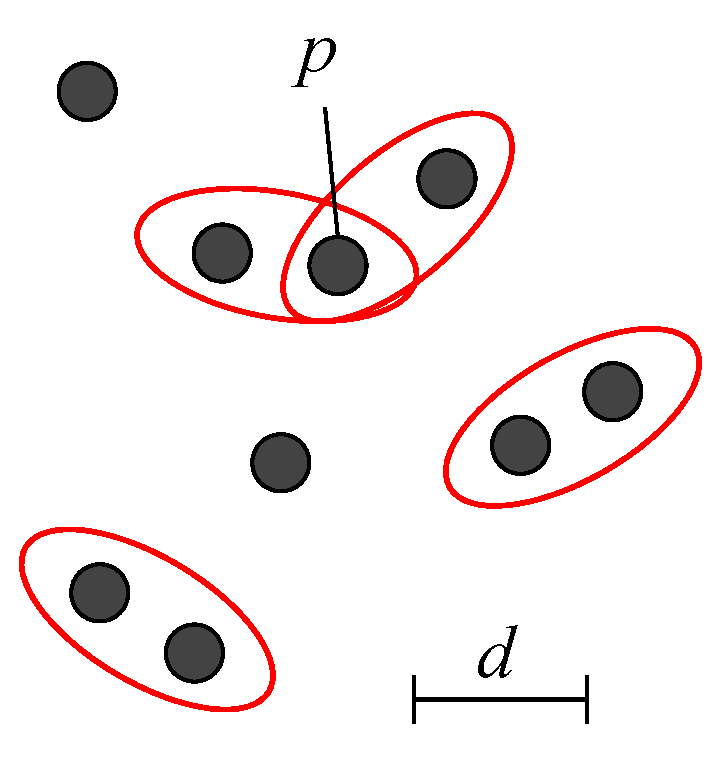
\includegraphics[scale=.3]{figs/cvl_proximity_conflicts.pdf}
\caption{Conflicts generated by the proximity constraint for distance $d$. Notice that point $p$ is a member of more than one \hl{conflict}.}
\label{fig:proximity:conflict}
\end{center}
\vspace*{-4ex}
\end{figure}

Consider a \hl{conflict involving} $k_1$ records, where at most $k_2$ of these records can be selected (where $k_1 > k_2$). Then it is equivalent to state that at least $\lambda = k_1 - k_2$ of these records must be \emph{deleted}. In the mathematical formulation of the problem in Section~\ref{sec:optimizationmodel}, we will use this alternative way to formulate \hl{conflicts}.

\subsection{\hl{Selection as an optimization problem}}
\label{sec:filtering}
\hl{The notion of conflicts is used to define the feasibility of solutions to the selection problem. This should be accompanied by a way to discriminate between solutions. Assigning an importance measure to each record, namely the record weights, intuitively allows us to measure the ``loss of importance'' due to records that are deleted.} 

\hl{In the optimization version of the problem, we seek the feasible solution that minimizes the aggregate weight of records that are deleted. In Section}~\ref{sec:optimizationmodel}\hl{, we present a mathematical formulation of the selection optimization problem}.

\hl{For a zoomable map with }$\mathcal{Z}$\hl{ zoom levels, we are interested in finding $\mathcal{Z}$ solutions to the selection problem, one for each zoom level }$i \in \lbrack 1, \mathcal{Z} \rbrack$. \hl{We call this problem the }\emph{multi-scale selection problem}. \hl{To control the way in which we compute these solutions, we use an algorithmic framework known as the }\emph{ladder} approach~\cite{foerster2010challenges}. \hl{This is a recursive approach, where the output of selection at large scale is used as input to selection at a smaller scale. This means that the zoom-consistency constraint }(Section~\ref{sec:constraints})\hl{ is automatically satisfied}.

\hl{The ladder approach is not appropriate for all use cases. For example, when regional labels are modeled as geospatial records, e.g., the label ``Europe'', we may wish to show a record only on intermediate zoom levels, violating zoom consistency. Handling these use cases would require an alternative formulation, e.g., following the }\emph{star} \hl{approach}~\cite{foerster2010challenges}. \hl{This is an interesting avenue for future work}.  

% should be visible mostly on the intermediate zoom levels, the }\emph{star} approach~\cite{foerster2010challenges}\hl{ would be better. This is a limitation of the work presented in this paper.}





% !TEX root = ./ICDE14_conf_full_296.tex
\section{CVL Language}
\label{sec:cvl:language}
The Cartographic Visualization Language (CVL) is a declarative language that can be used to specify an instance of the \hl{multi-scale selection problem} (Section~\ref{sec:filtering}). CVL is a rule-based language with a similar goal as other rule-based \hl{languages for selection over spatial datasets, i.e., to control the density of information at each zoom-level}~\cite{sld,mapnik}. The CVL approach is, however, markedly different. In the related languages, the user must explicitly control the \hl{selection} of records at each \hl{zoom level}, while also specifying how records are to be \hl{visualized}. First of all, CVL \hl{focuses only on selection, not presentation}. Furthermore, CVL controls \hl{selection} in a novel constraint-based way. Instead of having the user explicitly control the \hl{selection} of records at each \hl{zoom level}, CVL lets the user choose \emph{map constraints} that are instead enforced at all \hl{zoom levels}. By making the constraints explicit and the control implicit, a very concise formulation is obtained \hl{(see Figure}~\ref{fig:cvl:example:airports}\hl{ for an example)}.

CVL is one of the first languages and frameworks to implement the \hl{vision} of reverse data management~\cite{meliou2011reverse}. In reverse data management, the core idea is that a user states a set of constraints and an objective. These are given together with an input database to an optimization algorithm which computes an output database that is feasible and optimal with regard to the constraints and objective (if a feasible solution exists). This is exactly how CVL works. Furthermore, a feasible solution is guaranteed to exist, as \hl{deleting} all records is always a feasible solution.

The CVL language has two statements, the \emph{generalize} statement (see Section~\ref{sec:generalize:statement}) and the \emph{create-constraint} statement (see Section~\ref{sec:create:constraint:statement}). The create constraint statement is used to formulate new map constraints and the generalize statement is used to \hl{specify a solution to the multi-scale selection problem subject to those constraints.} 

The CVL language builds on top of SQL and reuses SQL as a language for formulating constraints and record weighting schemes.

\begin{figure}[!t]
\begin{center}
\begin{lstlisting}
GENERALIZE 
   {input} TO {output}
WITH ID {expression}
WITH GEOMETRY {expression}
AT {integer} ZOOM LEVELS
WEIGH BY
  {float expression}
SUBJECT TO 
   {constraint} {float parameters} [AND
   {constraint} {float parameters} [AND
   ...]]
\end{lstlisting}
\vspace*{-1ex}
\caption{Syntax of generalize statement.}
\label{fig:generalize:syntax}
\end{center}
\vspace*{-4ex}
\end{figure}

\subsection{Generalize statement}
\label{sec:generalize:statement}

\begin{figure*}[tb]
  \begin{minipage}{0.329\linewidth}
    \centerline{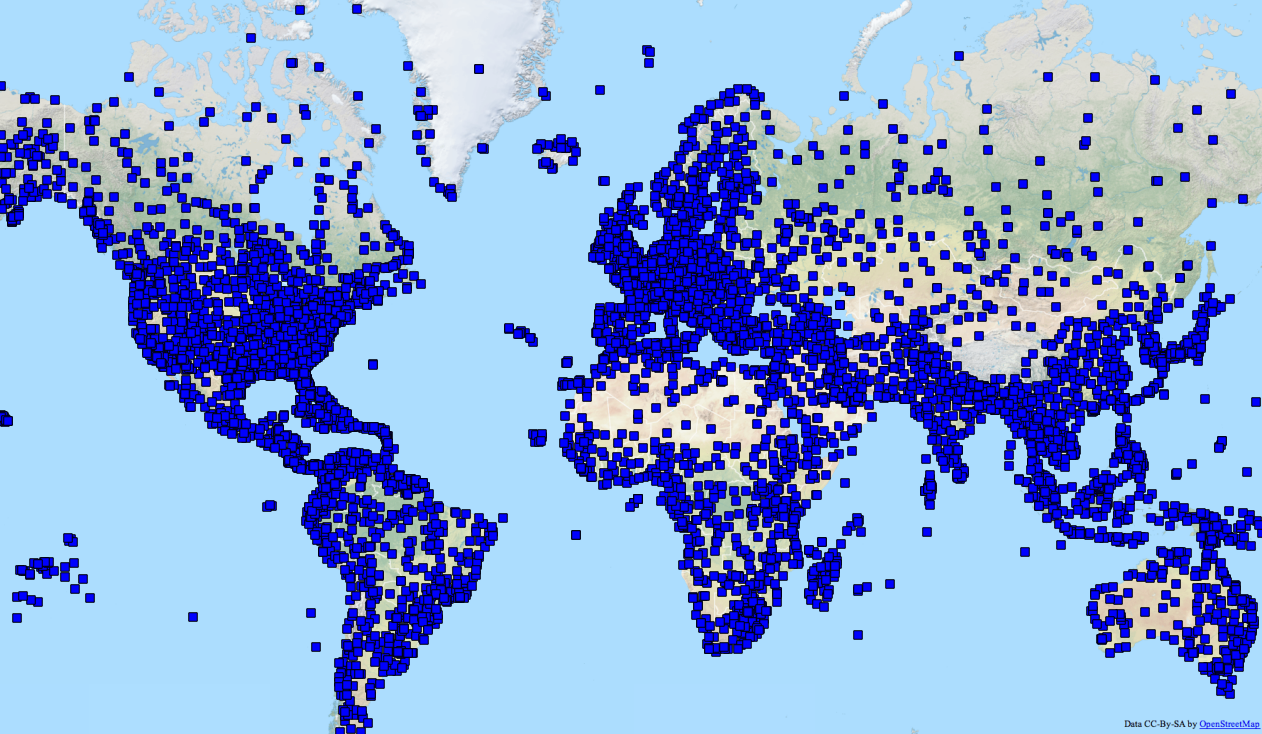
\includegraphics[width=0.95\linewidth]{./figs/airports.png}}
    \centerline{(a) Full Openflights Airport dataset}
  \end{minipage} \hfill
  \begin{minipage}{0.329\linewidth}
    \centerline{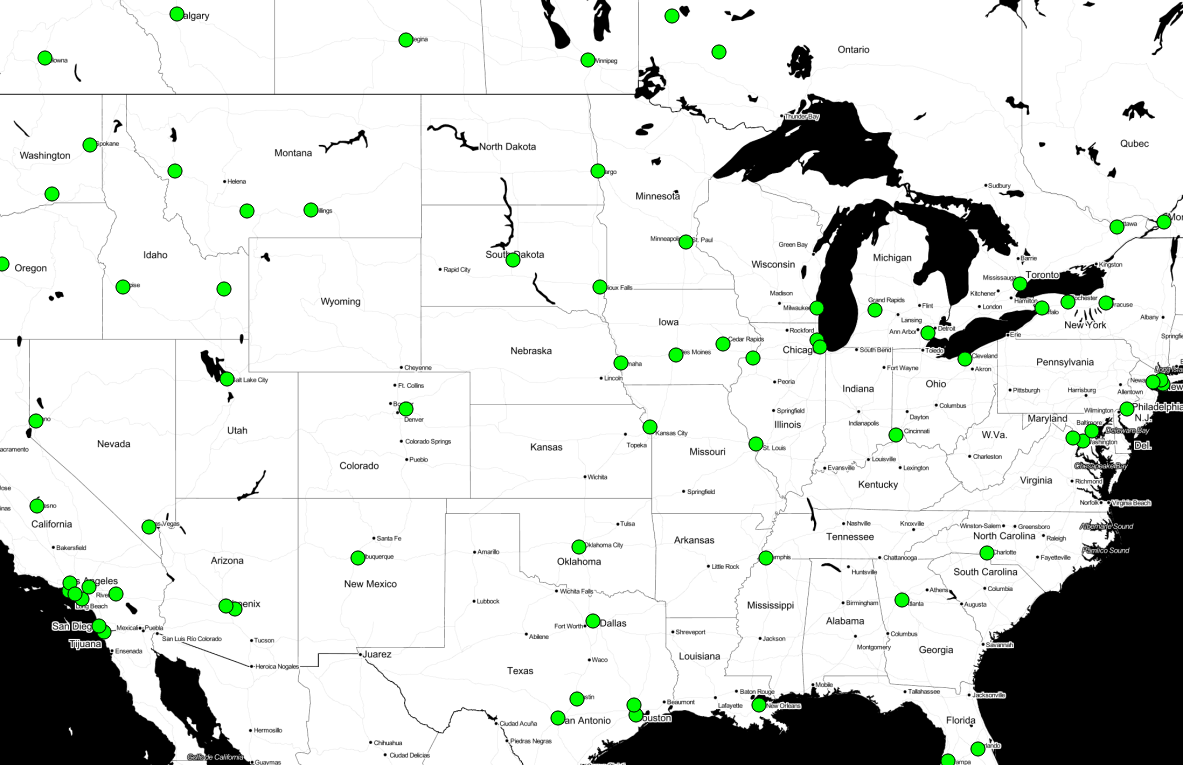
\includegraphics[width=0.95\linewidth]{./figs/airports_z4.png}}
    \centerline{(b) Airports on zoom-level 5}
  \end{minipage} \hfill
  \begin{minipage}{0.329\linewidth}
    \centerline{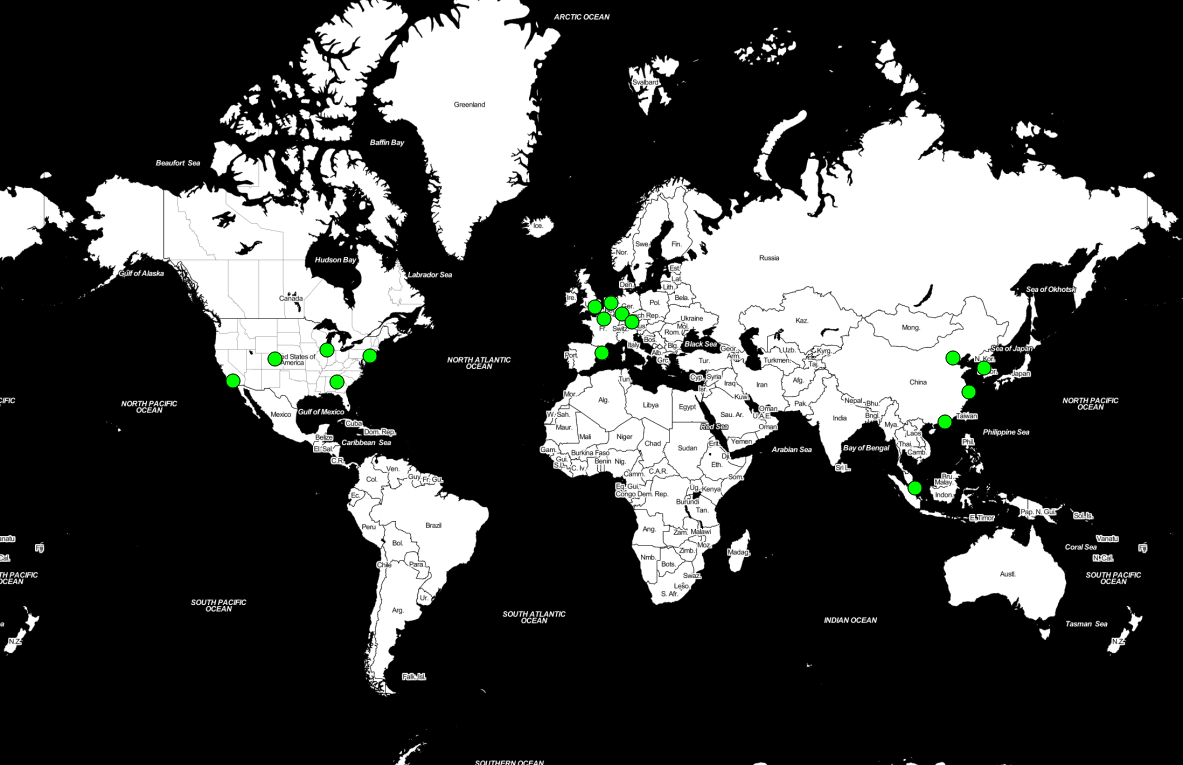
\includegraphics[width=0.95\linewidth]{./figs/airports_z0.png}}
    \centerline{(c) Airports on the top-most zoom-level.}
  \end{minipage}
  \vspace{-0ex}
  \caption{Airport map (7K points) before (a) and after (b, c) running CVL. The output corresponds to the CVL statement in Figure~\ref{fig:cvl:example:airports}.}
  \label{fig:graphical:output:airport}
  \vspace{-2ex}
\end{figure*}

The generalize statement is the main statement in CVL. This statement creates a new multi-scale dataset from an input table of geospatial records, subject to user defined constraints. The syntax is shown in Figure~\ref{fig:generalize:syntax}. The statement has several clauses, beginning with the specification of input and output tables. Instead of giving the name of an input table, the user can optionally write a select statement in SQL of the form \texttt{(SELECT ...) t}. \hl{The next clause is the }\emph{with-id}\hl{ clause, which is used to uniquely identify records. If records have an id column, this clause could simply provide the name of that column}. \hl{The }\emph{with-geometry}\hl{ clause is used to indicate the geometry property of records, e.g., the name of an available geometry column}. The next clause is the \emph{zoom-levels} clause where the user writes a positive integer, which is the \hl{highest zoom level} at which the \hl{selection} process will begin. The \emph{weigh-by} clause is used to give an arbitrary floating point expression that is evaluated for each row in the input and used as weight for that record. The \emph{subject-to} clause lists the map constraints along with any parameters (as a comma-separated list). The \texttt{AND} keyword is used to separate constraints in the case more than one is used.

%For clarity the syntax is shown without two clauses, the \emph{with-id} clause and the \emph{with-geometry} clause, which are used simply to specify the names of the ID and geometry columns in the input table.


An example of generalizing a dataset using the generalize statement is shown in \hl{Figures}~\ref{fig:graphical:output:airport}\hl{ and}~\ref{fig:cvl:example:airports}. In this example a dataset containing point records representing the location of airports world-wide is generalized \hl{(Figure}~\ref{fig:graphical:output:airport}\hl{(a))}. The records are weighted by using the name of a column containing the number of routes departing from each airport (\hl{shown in Figure}~\ref{fig:cvl:example:airports}; CVL automatically handles the cast from integer to floating point). The intuition is that airports with more departures are more important. The single constraint that is enforced is the visibility constraint, with a parameter of $K=16$. Recall that the visibility constraint says that each tile can contain at most $K$ records.


\begin{figure}[h]
%\vspace*{-2ex}
\begin{center}
\begin{lstlisting}
GENERALIZE 
   airports TO airports2
WITH ID airport_id
WITH GEOMETRY wkb_geometry
AT 18 ZOOM LEVELS
WEIGH BY
  num_departures
SUBJECT TO 
   visibility 16 
\end{lstlisting}
\vspace*{-1ex}
\caption{Generalization of an airports dataset. The airports are \hl{weighted} by number of departures. See Figure~\ref{fig:graphical:output:airport} for a vizualization of the result.}
\label{fig:cvl:example:airports}
\end{center}
\vspace*{-2ex}
\end{figure}



The resulting map is shown in Figure~\ref{fig:graphical:output:airport}\hl{(b) and~(c)} and has at most $16$ airports on each tile. For the single tile on the top zoom-level, the \hl{world's sixteen busiest airports are shown}. The CVL framework automatically gives priority to the airports with the highest weight. How this is done is explained in sections~\ref{sec:optimizationmodel} and~\ref{sec:algorithms}.

\subsection{Create constraint statement}
\label{sec:create:constraint:statement}

% change text
Map constraints are defined using the create-constraint statement.  The basic syntax of the statement is shown in Figure~\ref{fig:create:constraint:syntax}. The body of the statement is a SQL select statement that computes tuples that represent conflicts that are found at a given \hl{zoom level} in the map. \hl{A tuple }$\langle cid, rid\rangle$ denotes that record $rid$ is a member of conflict $cid$. See Section~\ref{sec:conflicts} for the \hl{exact semantics of conflicts}.

\begin{figure}[h]
\begin{center}
\begin{lstlisting}
CREATE CONSTRAINT C1
AS NOT EXISTS
  {SQL select statement}
  
RESOLVE cid IF DELETE (
  {integer expression}
)
\end{lstlisting}
%\vspace*{-1.5ex}
\caption{Syntax of create constraint statement}
\label{fig:create:constraint:syntax}
\end{center}
\vspace*{-1ex}
\end{figure}

\begin{figure}[htbp]
\begin{center}
\begin{lstlisting}
CREATE CONSTRAINT Proximity
AS NOT EXISTS (
  SELECT 
    l.{rid} || r.{rid} AS cid,
    Unnest(array[l.{rid}, r.{rid}]) AS rid
  FROM
    {level_view} l
  JOIN
    {level_view} r
  ON
    l.{rid} < r.{rid}
  AND
    l.{geom} && ST_Expand(r.{geom}, 
      CVL_Resolution({z}, 256) * 
        {parameter_1})
  AND
    ST_Distance(l.{geom}, r.{geom}) <
      CVL_Resolution({z}, 256) * {parameter_1}
)

RESOLVE cid IF DELETE (
  1
)
\end{lstlisting}
%\vspace*{-2ex}
\caption{Definition of the proximity constraint.}
\label{fig:proximity:definition}
\end{center}
\vspace*{-1ex}
\end{figure}

The \emph{resolve-if-delete} clause is used to compute the integer number of records that must be deleted in order to resolve the conflict with a given $cid$. 
%\hl{For the proximity constraint, this number is always 1, but for other constraints this may vary}.

Using this syntax, the definition of the proximity constraint is given in Figure~\ref{fig:proximity:definition}. The body of the constraint is a distance self join using a distance function \texttt{ST\_Distance} provided by a spatial extension to SQL. This join finds all pairs of records that are too close, e.g.\ less than $10$ pixels apart. For each conflict, the select statement outputs two tuples and exactly once for each conflict. The resolve-if-delete clause is simply the constant $1$, because that is how many records must be deleted to resolve a proximity conflict.

In Figure~\ref{fig:proximity:definition}, some names are enclosed in curly braces, such as \texttt{\{rid\}}. These are variables which are bound at runtime by the CVL framework and are intended for making the definition of constraints simpler. The variables \texttt{\{rid\}} and \texttt{\{geom\}} are bound to the column names containing the ID and geometry of the records. The \texttt{\{level\_view\}} is bound to a view that contains all records that are visible at the current level, i.e., the records that have not been filtered out at a higher zoom-level. The function \texttt{CVL\_Resolution(\{z\}, 256)} is one of the utility functions defined by the CVL runtime, also with the purpose of making the definition of constraints simpler. This function returns the resolution (meter/pixel) at zoom-level \texttt{\{z\}}, where \texttt{\{z\}} is a variable bound to the currently evaluated zoom-level. The variable \texttt{\{parameter\_1\}} is the constraint parameter, e.g. $10$ pixels.

\begin{figure}[htbp]
\begin{center}
\begin{lstlisting}
CREATE CONSTRAINT Visibility
AS NOT EXISTS (
    SELECT
        busted_tiles.cid,
        busted_tiles.rid
    FROM
        busted_tiles
)

RESOLVE cid IF DELETE (
  SELECT count(*) - {parameter_1}
  FROM   busted_tiles bt
  WHERE  bt.cid = cid
)

WITH SETUP (
    CREATE TEMPORARY TABLE busted_tiles AS (
        SELECT
            t.cid,
            Unnest(array_agg(t.cvl_id)) AS rid
        FROM
        (
        SELECT
            CVL_PointHash(CVL_WebMercatorCells({geometry}, {z})) AS cid,
            {rid}
        FROM
            {level_view}
        ) t
        GROUP BY t.cid
        HAVING count(*) > {parameter_1}
    );
    CREATE INDEX busted_tiles_id_idx ON busted_tiles (cid);
)

WITH TEARDOWN (
  DROP TABLE busted_tiles;
)
\end{lstlisting}
%\vspace*{-1.5ex}
\caption{Definition of the visibility constraint.}
\label{fig:visibility:definition}
\end{center}
%\vspace*{-3ex}
\end{figure}



Figure~\ref{fig:visibility:definition} shows how the visibility constraint may be defined using CVL. The CVL definition uses an extension of the basic create-constraint syntax, namely the \emph{setup} and \emph{tear down} clauses. 
%which will be covered again in Section~\ref{sec:implementation:extensions}. 
The purpose of these clauses is to enable arbitrary SQL statements to be run before and after the constraint body is evaluated at each zoom-level. During the setup phase we create an auxiliary table called \texttt{busted\_tiles} which contains tuples $\langle tile\_id, rid \rangle$ identifying tiles that are intersected by more than $K$ records, and the ID of those records. The body of the constraint simply iterates over the auxiliary table, using the \texttt{tile\_id} column as the conflict ID.




The user does not need to know how the conflicts are handled, because all conflicts are automatically resolved by the CVL framework using one of the algorithms presented in Section~\ref{sec:algorithms}.

%In this example, calls are made to other CVL runtime functions, namely \texttt{CVL\_WebMercatorCells} and \texttt{CVL\_PointHash}. These functions returns a set of points corresponding to the centroids of intersected tiles (given a geometry) and a unique identifier for points, respectively. The unique identifier for points is based on the well-known GeoHash algorithm.


% give the variables by example, and explain together with the example, instead of listing everything up front.

%\marcos{These could be introduced by need along with the examples integrated into the sections above.}


% !TEX root = ./cvl.tex
\section{\hl{Selection optimization problem}}
\label{sec:optimizationmodel}

In this section, we formally define the \hl{selection} problem as an optimization problem. Let $R$ be the set of records in the dataset. Each record $r \in R$ has an associated weight $w_r > 0$ which models the importance of the record. 

There are a number of constraints (formulated as conflict sets) that are modeled using CVL. Let $C$ be the collection of conflict sets. A conflict set $c \in C$ is a set of records $R_c \subseteq R$, where at least $\lambda_c \geq 1$ records must be deleted. 

\hl{The selection problem can now be modeled as a 0-1 integer program.} Let $x_r$ be a 0-1 decision for each record $r \in \bar{R}$ that is 1 if record $r$ is \emph{deleted}, and 0 otherwise. Then the single-scale problem can be stated as follows:

\begin{align}
  \label{eq:objective}
  \min ~\sum_{r \in R} &w_r x_r \\
  \label{eq:general-constraints}
  \sum_{r \in R_c} x_r &\geq \lambda_c, ~~~~ c \in C \\
  x_r & \in \{0, 1\}, ~~ r \in R, ~c \in C
\end{align}

The goal (\ref{eq:objective}) is to minimize the total weight of the records that are deleted. Constraints~(\ref{eq:general-constraints}) model the conflict sets $c \in C$. This is the \emph{set multicover problem} --- a generalization of the well-known set cover problem where each element/conflict set $c \in C$ needs to be covered $\lambda_c \geq 1$ times by the sets/records $r \in R$; each set/record can be chosen at most once~\cite{rajagopalan1998primal}.

\hl{While the set multicover problem is NP-hard, the selection optimization problem with conflicts is also NP-hard for all interesting cases. For an informal proof, consider the vertex cover problem. Given a graph $G=(V,E)$, find a minimum size subset of the vertices $S$ such that every edge in $E$ has an endpoint in $S$. Think of the vertices as records and the edges as conflict sets. This problem would then model the selection problem for the special case where all conflict sets had exactly two records (and all records had identical weights).

The vertex cover problem is NP-hard, even for very constrained cases. For example, even if $G$ is a planar graph and every vertex has degree at most 3, the problem remains NP-hard}~\cite{garey1977rectilinear}. \hl{In other words, even if the conflict sets only have two records each, and each record is involved in at most 3 conflict sets, the problem remains NP-hard. It is hard to imagine that any interesting application is more restrictive.

Note that the cubic vertex cover problem is APX-hard - which means that it cannot be approximated arbitrarily close unless $P=NP$}~\cite{alimonti2000some}. \hl{So even this restricted version is ``really'' hard.}

\hl{In the next section we discuss algorithmic approaches for solving the selection optimization problem. In the experimental evaluation of our approach we include a discussion on the objective value} (\ref{eq:objective}) \hl{of the selection optimization problem}.

% !TEX root = ./cvl.tex
\section{Algorithms}
\label{sec:algorithms}

\subsection{Algorithmic framework}

The algorithmic framework is illustrated in Figure~\ref{fig:algorithmic-framework}. After an initialization step, we solve $\mathcal{Z}$ single-scale optimization problems --- followed by a finalizing step.

\begin{figure}[htbp]
\begin{center}
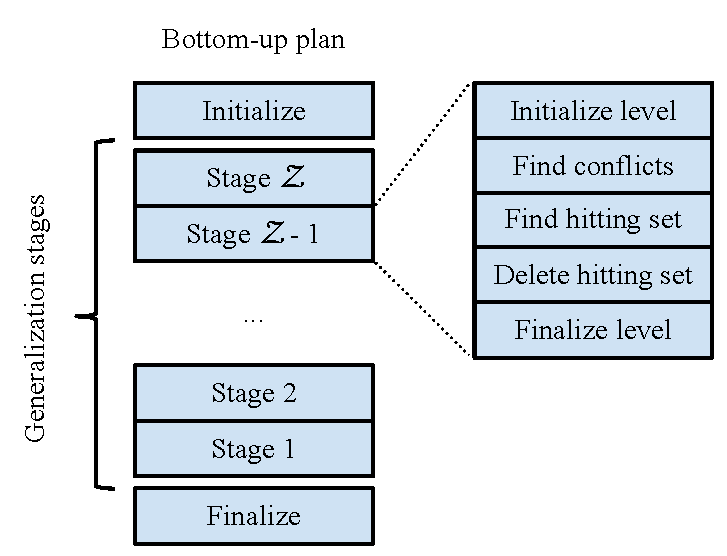
\includegraphics[scale=.6]{figs/cvl_stages.pdf}
\caption{The algorithmic framework: At stage $i$ the single-scale optimization problem is solved for the $i'th$ zoom level.}
\label{fig:algorithmic-framework}
\end{center}
\end{figure}

Below we describe three different heuristic algorithms for solving the single-scale optimization problem. Let $n=|C|$ be the number of constraints (or elements in the set multicover problem), and let $m=|R|$ be the number of records (or sets in the set multicover problem). Recall that $R_c \subseteq R$ is the set of records in constraint $c \in C$. The largest number of records in any constraint is $f = \max_{c \in C} |R_c|$, and is called the \emph{maximum frequency}.

\subsection{Static greedy algorithm (SGA)}

In this algorithm we consider each constraint $c \in C$ in turn, and simply choose the $\lambda_c$ records with minimum weight from constraint $R_c$ --- independently of what has been chosen earlier. If the sets $R_c$ are disjoint, the algorithm is clearly optimal. However, in general no approximation guarantee can be provided. The algorithm runs in $O(n f \log f)$ time, as we just need to sort the records by weight for each constraint; alternatively we can sort all records by weight in $O(m \log m)$ time and pick the minimum weight records from the constraints in linear time in the total number of records in all constraints.

\subsection{LP-based greedy algorithm (LPGA)}

In this algorithm we first solve a linear programming (LP) relaxation of the set multicover problem. This LP-problem is obtained by relaxing the constraint $x_r \in \{0, 1\}$ to $0 \leq x_r \leq 1$. Then we choose all records $r \in R$ for which the LP-solution variable $x_r$ is at least $\lambda_c / f$ (for some constraint $c \in C$ where $r \in R_c$). Intuitively, we round up all fractional values that are large enough. 

This algorithm provides a feasible solution to the single-scale problem, and the approximation guarantee is $\max_{c \in C} f / \lambda_c$~\cite{something}; thus, if $f$ is small, the algorithm provides a good approximation guarantee. As the LP-problem can be solved in polynomial time, the complete algorithm is polynomial.

\subsection{Dynamic greedy algorithm (DGA)}

Described in Vazirani 13.2.1. @Martin: Please write here.

\marcos{I would only introduce DGA if it is actually evaluated in the experiments.}



% !TEX root = ./cvl.tex

\section{Implementation}
\label{sec:implementation}

In this section, we present how our implementation makes use of in-database execution to provide scalability and engine reuse for CVL (Section~\ref{sec:implementation:indatabase}). In addition, we discuss a number of extensions to CVL that we found to be useful for practical applications (Section~\ref{sec:implementation:extensions}). 

\subsection{In-Database Execution}
\label{sec:implementation:indatabase}

\minisec{Overview}
Since CVL is declarative, and CVL constraints are already expressed in SQL, it is natural to attempt to reuse as much existing DBMS technology as possible to execute CVL. Figure~\ref{fig:indatabase} shows how CVL is compiled for execution in a relational DBMS, which acts as the language runtime. The output of the CVL compiler is a database script for the target host, containing both SQL and stored procedures, and following the algorithmic framework of Figure~\ref{fig:algorithmic-framework}. The script is pushed down to the database engine, and operates against the appropriate input data stored in the system. This strategy offers us two main advantages:

\begin{enumerate}

\item Since all code is pushed down and both input and output reside in the database, we do not need to transfer any data outside of the database engine. This co-location of code and data is a significant advantage for large datasets.

\item By expressing as much as possible of the generated code in SQL, we can reuse decades of optimizations built into database engines, especially for geospatial data~\cite{Guttman1984:RTree,Hellerstein1995:GiST}. This opens up many opportunities, such as automatic optimization, parallelism, and selection of specialized algorithms and indexes.  

\end{enumerate} 

While the general strategy of compiling declarative languages to SQL has been pursued in other contexts, e.g., for XQuery~\cite{pathfinder} and LINQ~\cite{ferry}, our context poses a particular challenge of integrating the language with algorithmic solvers inside the database. 

\begin{figure}[htbp]
\begin{center}
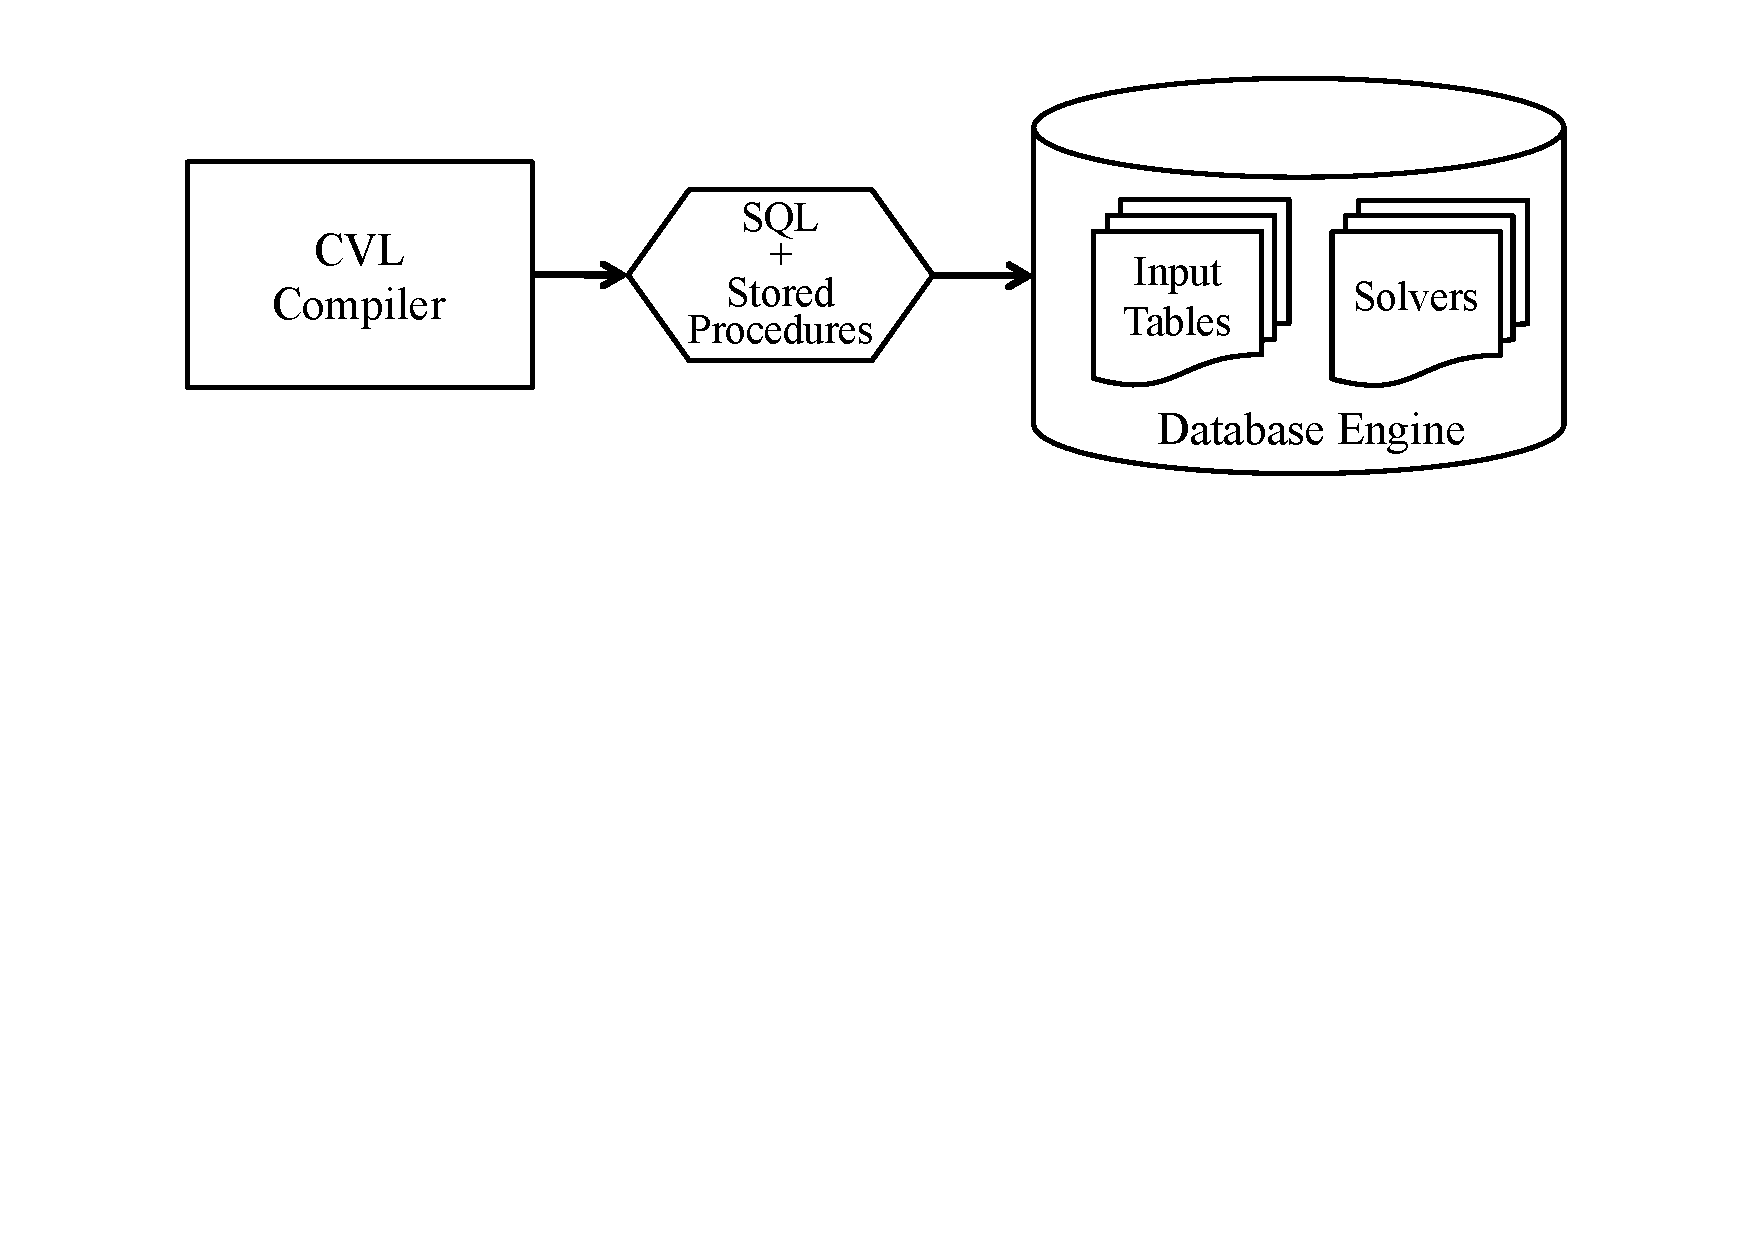
\includegraphics[scale=.35,viewport=400 375 450 550]{figs/indatabase-execution.pdf}
\caption{CVL and in-database execution.}
\label{fig:indatabase}
\end{center}
\end{figure}

\minisec{Solvers}
In Section~\ref{sec:algorithms}, we have presented two different algorithmic approaches for solving CVL generalizations: static greedy (SGA) and LP-based greedy (LPGA). We now show how to express each of these approaches in SQL along with stored procedures. 

SGA is the simplest algorithm, and recall that it operates independently on the conflicts generated by each constraint. Suppose the conflicts $\bar{C}$ generated by the active constraints are stored in a \emph{conflicts} table. Then for conflict set $c \in \bar{C}$, SGA is tantamount to the query:

\begin{lstlisting}
SELECT rid
FROM (
  SELECT ROW_NUMBER() 
         OVER (PARTITION BY cid
               ORDER BY cvl_rank) AS r,
         rid, cvl_rank, lambda_c
  FROM conflicts) h
WHERE h.r <= h.lambda_c
\end{lstlisting}

For each conflict set $c$, we order records by rank, and ensure that we pick at least $\lambda_c$ records. The declarative formulation allows us to reuse optimized sorting code in the database engine for execution.

LPGA solves a linear programming relaxation of the set multicover problem. We express LPGA by a stored procedure. The procedure accesses the conflicts for the constraints via SQL, constructs an appropriate LP, and then calls into an LP solver library~\cite{cvxopt}. Since the solver library does not use built-in database optimizations, this execution strategy for LPGA only leverages the first advantage of data and code co-location listed above.

Finally, note that the code for finding conflict sets is already expressed in SQL by the user for each constraint. As a consequence, this user code can make use of all built-in database optimizations available in the target engine.

%\minisec{CVL runtime functions}
%In the definition of the visibility constraint in Section~\ref{sec:create:constraint:statement} we reference two stored procedures in the CVL runtime library, \texttt{CVL\_PointHash} and \texttt{CVL\_WebMercatorCells}. These functions are implemented in SQL and make use of the spatial extension of the database~\cite{postgis}.

%The procedure \texttt{CVL\_PointHash} uses a call to \texttt{ST\_GeoHash} to implement an injective mapping from points to strings. The GeoHash algorithm corresponds to a Z-order curve, and we exploit this for uniquely naming tiles when evaluating the visibility constraint, i.e. finding tiles with more than $K$ records.

%The \texttt{CVL\_WebMercatorCells} function maps a geometry at a given zoom-level to centroids of all intersected tiles (on that zoom-level). We experimented with several ways to do this for general geometries (points, line segments, polygons) and found that rasterizing the geometry (using the function \texttt{ST\_AsRaster} in the spatial extension of the database) and iterating over the indices was the fastest for general geometries. For point records it is significantly faster to use the standard transformation function \texttt{ST\_SnapToGrid}.

%An improvement to \texttt{CVL\_WebMercatorCells} that we did not have time to implement is to compute tiles as quad-keys on the highest level only. Tile identifiers for lower levels are easily computed by taking prefixes of the quad-keys. This approach only benefits the running time when using constraints that are tile-based.

\subsection{Extensions}
\label{sec:implementation:extensions}

When designing CVL, we realized a number of our interesting use cases for the language that we had not initially considered. This realization, along with our implementation experience of CVL use cases, led us to a set of extensions over the core language targeted at improving convenience of use. We present these extensions below.

\minisec{Partitioning and Merging Datasets} 
A single input table may contain geospatial objects of different classes, e.g., roads and points of interest. When this is the case, users often wish to generalize some of these classes of objects independently, but obtain a single result map. While this can be done by merging the results of multiple GENERALIZE statements, we found it useful to add syntactic sugar to support this case. We extend the GENERALIZE statement with PARTITION BY and MERGE PARTITIONS clauses. PARTITION BY allows us to effectively segregate the input into multiple independent sets. MERGE PARTITIONS combines a few of these sets back together before providing them as input to generalization. For example, assume a \emph{geo\_objects} table contains highways, roads, restaurants, and hotels, tagged by a \emph{type} attribute. We could then generalize \emph{geo\_objects} as follows:

\begin{lstlisting}
GENERALIZE  geo_objects
TO network_and_poi_map
...
PARTITION BY type
MERGE PARTITIONS 'restaurant', 'hotel' 
              AS 'poi'
... 
\end{lstlisting}

In the example, we overlay independent generalizations of highways, roads, and points of interest into a single map. However, restaurants and hotels are generalized as a single input set.  

\minisec{Forced and All-or-Nothing Visualization}
Intuitively, constraints let users specify what is \emph{not} allowed in a given map, by forbidding the existence of conflicts. However, users also find helpful to control certain behaviors that \emph{must} occur in their map. We extended the GENERALIZE statement with support for two types of behaviors: (1)~the ability to mandate a minimum zoom level for a particular partition of the input, and (2)~the ability to force that either all or none of the objects of a given partition be displayed. For example, a user may wish to specify that highways must only appear at zoom level 10 or lower in their map. In addition, for consistency, either the whole highway skeleton is displayed or no highways should show up. To achieve this goal, we extend the GENERALIZE statement by a FORCE clause with MIN LEVEL and ALLORNOTHING specifiers. Continuing the example above:

\begin{lstlisting}
...
FORCE MIN LEVEL 10 ALLORNOTHING FOR 'highway'
... 
\end{lstlisting}

In the evaluation of CVL, the minimum level specifier controls what data is given as input for a zoom level. The all-or-nothing specifier, on the other hand, controls filtering of the output of the level generalization process. If the specifier is present, all records of a partition are eliminated if any record from the partition input is not present in the output. By filtering output, we ensure that the result also respects all other constraints specified by the user. 

%\minisec{Set up and Tear Down for Constraints}   
%Map constraints can exhibit significant complexity. Since a constraint is expressed as a single SELECT statement, it is often helpful to be able to refer to temporary tables in its formulation. We have thus extended the CREATE CONSTRAINT statement to include two additional clauses: WITH SETUP and WITH TEARDOWN. The former allows a user-defined SQL statement to be executed in advance of the constraint evaluation, creating any supporting tables for the evaluation of the constraint. The latter specifies user-defined cleanup code. Note that since constraints are evaluated independently at each zoom level, the set-up and tear-down clauses are evaluated before and after the constraint SQL at each zoom level.       
%\marcos{Move necessary information from paragraph above to Language section, and remove paragraph after that.}

%
% MVS: We can probably get away with not showing the syntax below. 
%
%\begin{lstlisting}
%CREATE CONSTRAINT C1 
%AS NOT EXISTS
% (SELECT cid, rid, minhits
%  FROM {more SQL})
%WITH SETUP
% {user-defined SQL}
%WITH CLEANUP
% {user-defined SQL}
%\end{lstlisting}



% !TEX root = ./cvl.tex
\section{Experimental Results}
\label{sec:experimental}

\martin{Compare experimental results with theory e.g. expected approximation guarantee, number of constraints, number of records per constraint etc.}

In this section, we present experimental results with our implementation of CVL. Our experiments have the following goals:

\begin{itemize}

\item Evaluate the performance and solution quality of CVL generalizations with a variety of real-world datasets, including point data as well as complex shapes such as polygons and line strings. 

\item Analyze the performance and solution quality of CVL generalizations produced under the proximity and visibility constraints presented in Section~\ref{sec:cvl:language} by both the SGA as well as the LPGA solvers of Section~\ref{sec:algorithms}.

\item Observe how the performance of CVL with different constraints and solvers scales with the number of objects in the geospatial dataset.

\end{itemize}

We start by presenting our experimental setup (Section~\ref{sec:exp:setup}), and then show results for both point data (Section~\ref{sec:exp:points}) and complex shapes (Section~\ref{sec:exp:complex:shapes}). Each result section discusses performance, quality, and scalability. 


\subsection{Experimental Setup}
\label{sec:exp:setup}

\minisec{Datasets}
We have tested CVL using four real-world datasets with the biggest one containing 23 million points and one synthetic dataset containing 30 million points. We list all datasets in Table~\ref{tab:datasets}. 

We have used three point datasets. The airports dataset is from Openflights~\footnote{\texttt{http://openflights.org/data.html}} and contains 7411 airports (points). The tourism dataset contains 500 thousand points representing tourist attractions worldwide from the OpenStreetMap database~\footnote{\texttt{http://www.openstreetmap.org/}}. The fractal dataset (synthetic) was created by iteratively copying and displacing points from the tourism dataset within a 10km radius until 30 million records were reached.

We have used two line segment datasets. The US rivers/streams dataset contains roughly 4 thousand rivers and roughly 27 thousand streams in the United States derived from the OpenStreetMap database. Records with identical name attributes have been merged into one. In the original dataset, most rivers are represented by multiple records, which is unfortunate in a filtering situation (either show the waterway completely or not at all). 

We have used a single polygon dataset, the area information dataset~\footnote{\texttt{http://internet.miljoeportal.dk/}} from The Danish Natural Environment Portal, published by the Danish government. This dataset contains 30 thousand high-fidelity administrative protection zone polygons, and ranging from small polygons the size of buildings to large polygons the size of entire regions. The biggest polygon is described by more than 36 thousand points.

\begin{table}[htdp]
\caption{Datasets used in experiments}
\label{tab:datasets}
\begin{center}
\begin{tabular}{|c|c|c|c|c|}
\hline
\textbf{Origin} & \textbf{Dataset} & \textbf{Type} & \textbf{Records} & \textbf{Points} \\
\hline
Real & Airports & Points & $7K$ & $7K$ \\
Real & Tourism & Points & $500K$ & $500K$ \\
Synthetic & Fractal & Points & $30M$ & $30M$ \\
Real & US rivers & Line segments & $4K$ & $2M$ \\
Real & US rivers/streams & Line segments & $30K$ & $6M$ \\
Real & Proctection zones & Polygons & $30K$ & $9M$ \\
\hline
\end{tabular}
\end{center}
\label{default}
\end{table}%


\minisec{Hardware, Software, and Methods}
The machine used for testing was an Amazon EC2 instance with 17GB RAM, 2 x Intel(R) Xeon(R) CPU E5-2665 0 @ 2.40GHz and 20MB Cache, running Amazon Linux 3.4.48-45.46.amzn1.x86\_64\footnote{An image of the instance we used for testing is available through Amazon EC2 as an AMI. The image contains the exact database used for testing, with all tables preloaded}.

The database used for testing was PostgreSQL 9.2.4 with PostGIS  2.0 built against the following libraries: GDAL 1.9.2 and GEOS 3.3.8. For the LP solver we integrated the database with the convex optimization library CVXOPT version 1.1.6~\cite{cvxopt}. We installed Python language bindings in the database against Python 2.6.8.

We ran each test three times on this installation, taking averages. We observed that measurements were very stable, with negligible difference in compute time between runs.

PostgreSQL always uses a single core to compute a transaction. Because the generalization process in CVL runs as a single long transaction, each job in CVL runs on a single core. A future direction would be to investigate parallel execution of CVL queries using a different language runtime such as a parallel database or a MapReduce environment.

\minisec{Sweep-line approach for varying dataset size}

We have tested the scalability of CVL using both point and line segment datasets. For this we needed a way to gradually increase the size of a dataset, without affecting density too much.  For this we used a line sweep approach. First, we ordered records by minimum x-coordinate, and then used increasingly large prefixes of this order to derive bigger datasets. The advantage of this approach over random sampling is that the spatial density of records is better preserved.

\minisec{Average optimality ratio}
In our approach we solve the multi-scale filtering problem as a series of single-scale filtering problems. Ideally we would like to compare the objective value of our multi-scale solution to a lower bound or an optimal solution to the multi-scale filtering problem. However, due to the scale of the multi-scale problem, we have not developed a method for computing a lower bound or an optimal solution.

In order to get an indication of solution quality, we have instead compared the solutions to the single-scale filtering problems to the lower bounds coming from solving the LP-relaxation of the integer program for the single-scale filtering problem. The numbers we present in Table~\ref{tab:points:overview} and Table~\ref{} are obtained by computing the average ratio between our solution value and the corresponding lower bound for each zoom level. 

\subsection{Point Data}
\label{sec:exp:points}

In this section, we present experimental results with point datasets, namely the Openflight airports and Tourist attractions datasets. We first discuss performance and quality for CVL and then proceed to analyze CVL's scalability behavior. Even though we experimented with all combinations of solvers (SGA / LPGA) and constraints (visibility / proximity / combined), we show only representative results for brevity. Results for the combined visibility and proximity constraints exhibited the same performance trends as of the most expensive of the two constraints. All other results followed similar trends as the ones explored below.

\begin{figure*}[tb]
  \begin{minipage}{0.329\linewidth}
    \centerline{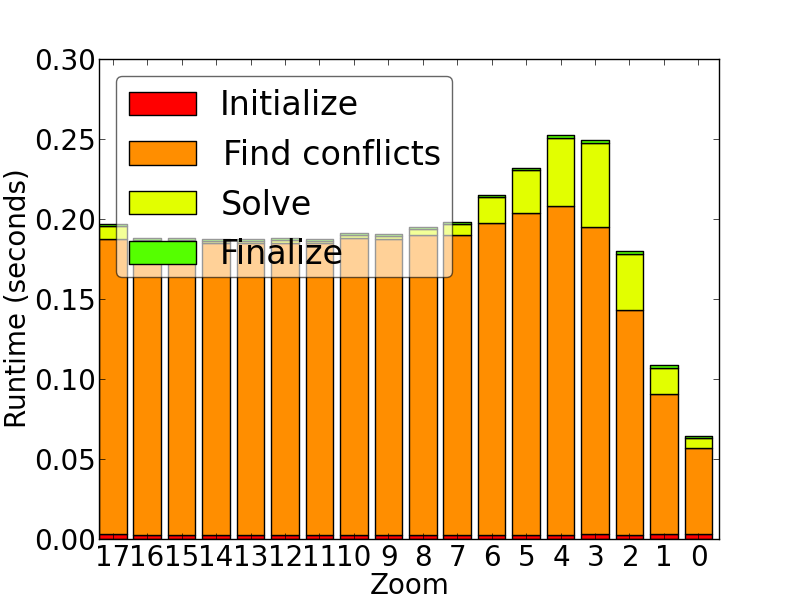
\includegraphics[width=1.0\linewidth]{./figs/prelim_pnt_7k_airports_heuristic_B.png}}
    \centerline{(a) SGA + Proximity}
  \end{minipage} \hfill
  \begin{minipage}{0.329\linewidth}
    \centerline{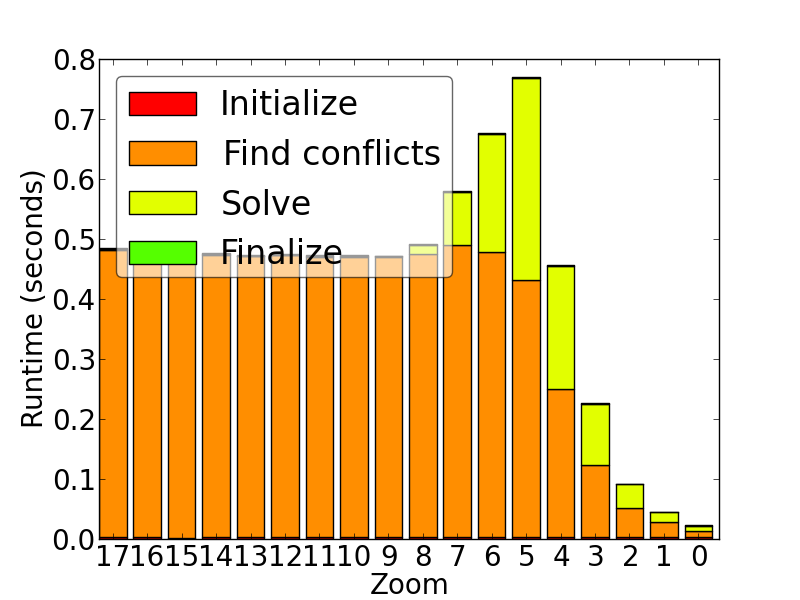
\includegraphics[width=1.0\linewidth]{./figs/prelim_pnt_7k_airports_lp_A.png}}
    \centerline{(b) LPGA + Visibility}
  \end{minipage} \hfill
  \begin{minipage}{0.329\linewidth}
    \centerline{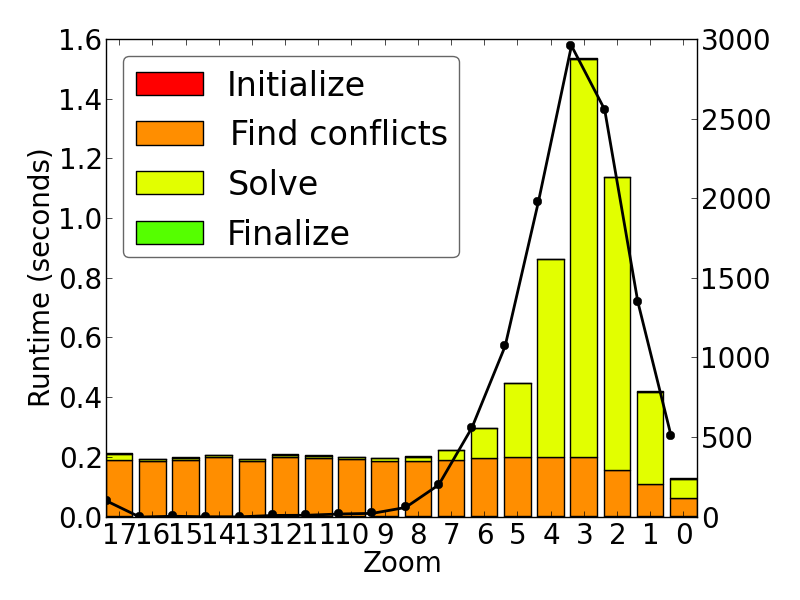
\includegraphics[width=1.0\linewidth]{./figs/prelim_pnt_7k_airports_lp_B.png}}
    \centerline{(c) LPGA + Proximity}
  \end{minipage}
  \vspace{-0ex}
  \caption{Performance breakdown by zoom level, Airport dataset (7K points). The black line indicates number of conflicts} \label{fig:performance:airport}
  \vspace{-2ex}
\end{figure*}

\begin{figure*}[tb]
  \begin{minipage}{0.329\linewidth}
    \centerline{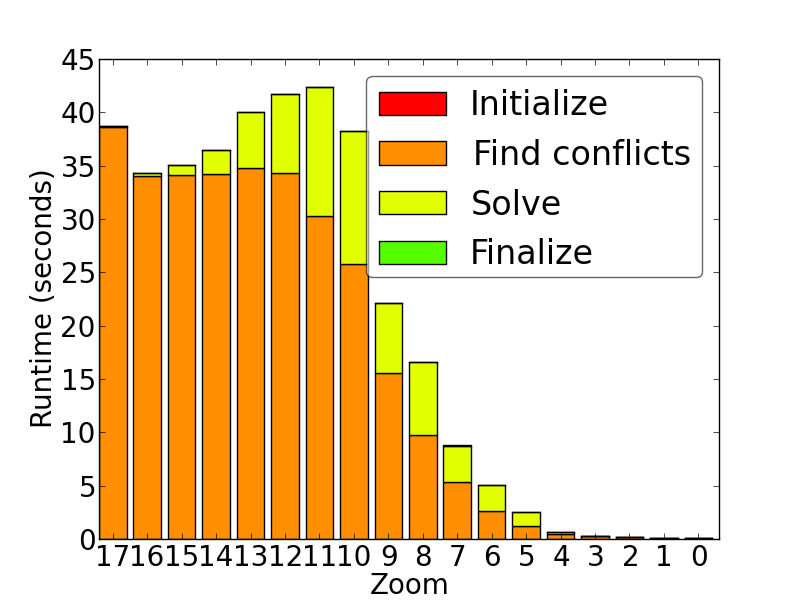
\includegraphics[width=1.0\linewidth]{./figs/prelim_pnt_500k_tourism_heuristic_A.png}}
    \centerline{(a) SGA + Visibility}
  \end{minipage} \hfill
  \begin{minipage}{0.329\linewidth}
    \centerline{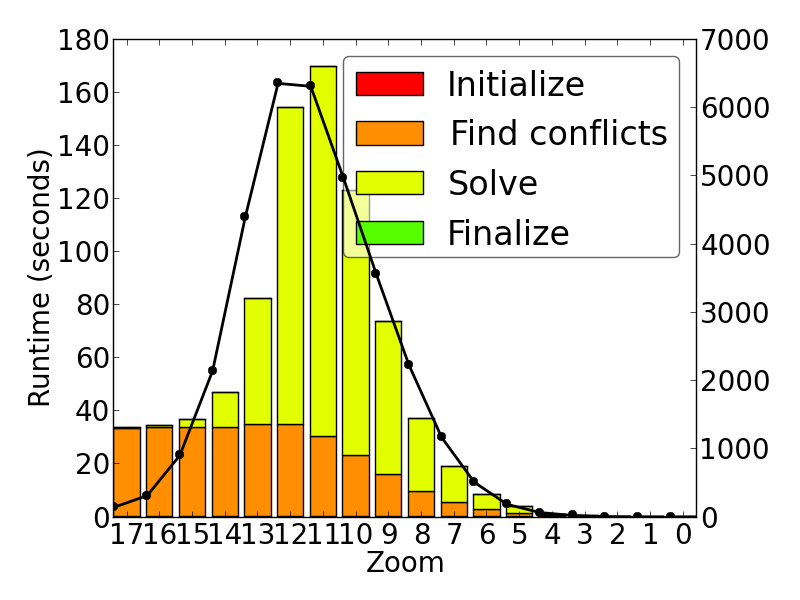
\includegraphics[width=1.0\linewidth]{./figs/prelim_pnt_500k_tourism_lp_A.png}}
    \centerline{(b) LPGA + Visibility}
  \end{minipage} \hfill
  \begin{minipage}{0.329\linewidth}
    \centerline{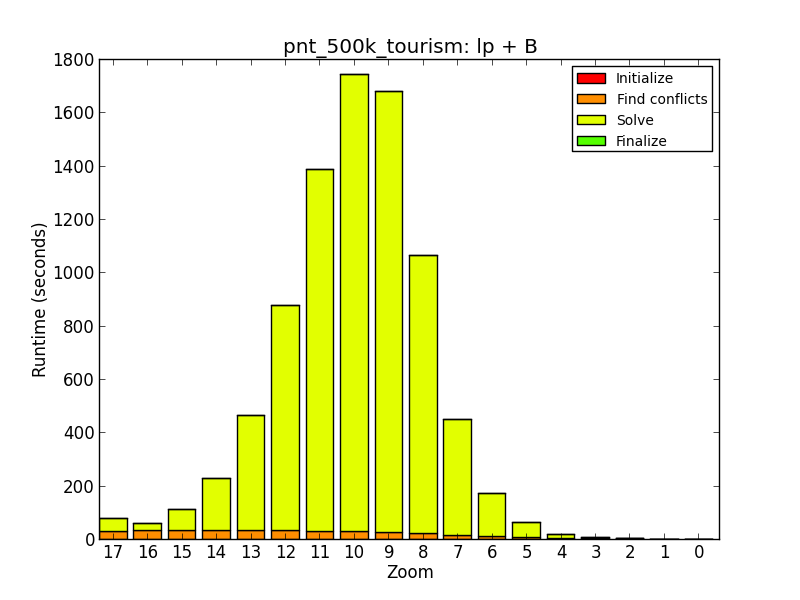
\includegraphics[width=1.0\linewidth]{./figs/prelim_pnt_500k_tourism_lp_B.png}}
    \centerline{(c) LPGA + Proximity}
  \end{minipage}
  \vspace{-0ex}
  \caption{Performance breakdown by zoom level, Tourism dataset (500K points). The black line indicates number of conflicts} \label{fig:performance:tourism}
  \vspace{-2ex}
\end{figure*}

\minisec{Performance and quality}
An overview of running times and solution qualities for the point datasets are shown in Table~\ref{tab:points:overview}. In Section~\ref{sec:algorithms:sga} we wrote that SGA is optimal for disjoint conflict sets. This is confirmed by the entries for visibility + SGA in the table. For the point datasets we used for testing, the LPGA algorithm is also optimal or within $3\%$ of the optimum when combined with the visibility constraint, probably cause by the conflict sets being disjoint. Recall that the approximation guarantee of LPGA is $f$, see Section~\ref{sec:algorithms:lpga}.

In terms of quality, the difference between SGA and LPGA is not stark, and depends more on the constraint than on the solver, with visibility generally yielding the best solutions.

\begin{table}[htdp]
\caption{Results for CVL on point datasets grouped by constraint}
\begin{center}
\begin{tabular}{|c|c|c|c|c|}
\hline
\textbf{Dataset} & \textbf{Constraint} & \textbf{Solver} & \textbf{Time} & \textbf{Avg. opt. ratio}\\ 
\hline
Airports (7K) & Visibility & SGA & 7s & 1.0 \\
Airports (7K) & Visibility & LPGA & 7s & 1.03 \\
Tourism (500K) & Visibility & SGA & 6m 9s & 1.0 \\
Tourism (500K) & Visibility & LPGA & 13m 35s & 1.0 \\
\hline
Airports (7K)  & Proximity  & SGA & 3s & 1.18 \\
Airports (7K)  & Proximity & LPGA & 7s s & 1.22 \\
Tourism (500K) & Proximity & SGA & 7m 17s & 1.21 \\
Tourism (500K) & Proximity & LPGA & 2h 18m & 1.24 \\
\hline
\end{tabular}
\end{center}
\label{tab:points:overview}
\end{table}%

Figure~\ref{fig:performance:airport} shows the performance breakdown per zoom level of executing CVL with the Openflight airports dataset. Note the different y-scales in the graphs. We have overlayed the number of conflicts per zoom-levels as a black line. In Parts~(a)-(c), we observe that the time needed to find conflicts is roughly stable until eight zoom levels, then slightly increases, and finally drops sharply for lower zoom levels. The constraints used generate few conflicts at higher zoom levels, given the relatively low density of the airport distribution in space. Nevertheless, even though almost no conflicts are generated, the dataset is still processed, resulting in roughly equal time for finding conflicts and negligible time for solving conflicts per zoom level. 
 
As zoom levels decrease, more conflicts naturally arise, leading initially to increased conflict finding time, as well as conflict solving time. However, as conflicts are solved, records are deleted from the dataset taken as input for the next zoom level. This procedure causes conflict finding time (and eventually total time) to drop significantly for low zoom levels. For SGA under the proximity constraint (Part (a)), total time at zoom level zero is over two times shorter than the initial runtime at zoom level 17; for LPGA under the visibility constraint (Part (b)), the difference in total time reaches over an order of magnitude.  

Conflict solving time does not increase equally for different solvers. SGA exhibits conflict solving time that is consistently smaller than LPGA. Peak total time for SGA under the proximity constraint (Part (a)) is roughly four times shorter than for LPGA (Part (c)). In addition, LPGA is extremely sensitive to the number of conflicts reported by user-defined constraints. From Parts (b) and (c), we can see that LPGA exhibits peak conflict solving time over three times larger for the proximity constraint than for the visibility constraint, since the latter generates far fewer conflicts than the former.

Figure~\ref{fig:performance:tourism} exhibits results with the larger tourism attraction dataset. Since the dataset is denser in space than the airport dataset, conflicts are found and solved at higher zoom levels, resulting in an earlier drop in total time per zoom level. For Parts (a)-(c), total time is uninteresting for zoom levels lower than five. The same cannot be said, however, about peak total time in general, and about conflict solving time in particular.

Parts (a) and (b) compare performance of SGA and LPGA under the visibility constraint. Even though visibility generates a smaller number of conflicts than proximity, peak total time for LPGA is still roughly a factor of four larger than for SGA (see zoom level 11). Note that the difference is completely due to the efficiency of the solver, since the time to find conflicts is essentially the same for both methods. Total time for LPGA rises prohibitively when we employ the proximity constraint, reaching a baffling peak of near half an hour at zoom level 10 (Part (c)). While not shown, total times per zoom level for SGA under the proximity constraint are roughly comparable to the times reported in Part (a) for the visibility constraint using this dataset. SGA's peak total time is slightly above 40 seconds, roughly a factor of 40 smaller than LPGA's.         

While SGA performs significantly better than LPGA, it does not do so at the cost of quality, at least for point datasets. As discussed in Section~\ref{sec:algorithms:sga}, SGA is optimal for the visibility constraint, since conflict sets are disjoint. For the proximity constraint, we observe that the solutions have comparable quality for the two algorithms, while the running time of LPGA is much larger than SGA, and more so for the larger dataset.

\minisec{Scalability}
We tested the scalability of CVL by varying the size of the synthetic dataset of 30 million points, starting with one thousand records, and tested by iteratively doubling up until we reached roughly four million records. We used the sweep-line approach introduced in Section~\ref{sec:exp:setup} to increase the dataset size. We have plotted the running time of each solver/constraint combination for different dataset size in Figure~\ref{fig:scalability}.

In general, we found that SGA scales a lot better than LPGA, which confirms the observation we made in the performance breakdown above. After reaching four million points the running time became prohibitively large (more than 3 hours) even for SGA. Up to this point the algorithm scales more or less linearly. The running time of the solvers depend on the number of conflicts, as well as the structure of the conflicts. It is easy to see that after the first zoom-level, the number of conflicts is bounded by a constant that is proportional either on the number of records (for the proximity constraint) or the number of cells (for the visibility constraint). For the proximity constraint each point can be in at most six conflicts. For the visibility constraint, each cell can contain at most $64$ records for $K=16$, after the first zoom-level is processed.

There is a curious fall in running time for SGA with the proximity constraint. We did not gather sufficient data during the scalability experiment to explain this phenomenon.

\begin{figure*}[tb]
  \begin{minipage}{0.49\linewidth}
    \centerline{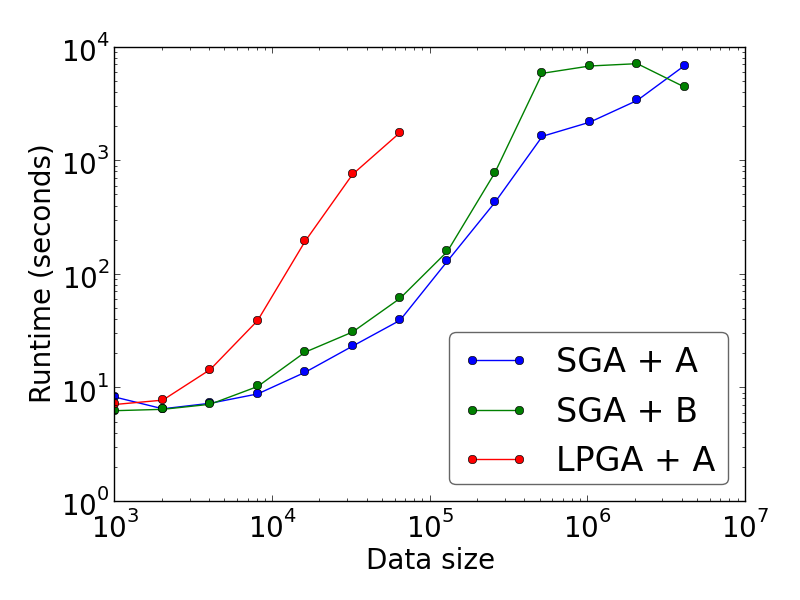
\includegraphics[width=0.9\linewidth]{./figs/scal_pnt_30m_synthetic.png}}
    \centerline{(a) Scalability for point data}
  \end{minipage} \hfill
  \begin{minipage}{0.49\linewidth}
    \centerline{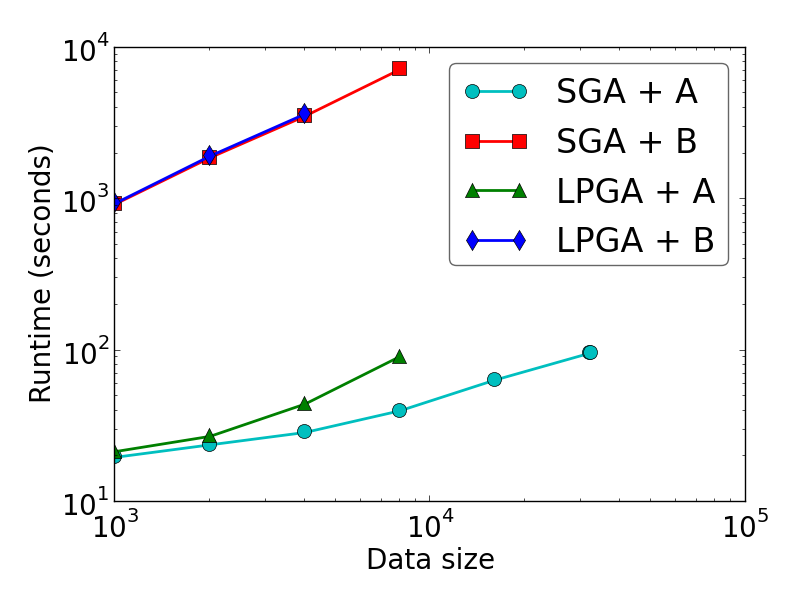
\includegraphics[width=0.9\linewidth]{./figs/scal_lin_30k_uswaterway.png}}
    \centerline{(b) Scalability for complex shape data}
  \end{minipage} \hfill
  \vspace{-0ex}
  \caption{Scalability of CVL for point datasets and complex shape datasets. Constraints are marked as \emph{Visibility}: A, \emph{Proximity}: B} \label{fig:scalability}
  \vspace{-2ex}
\end{figure*}

\subsection{Complex Shape Data}
\label{sec:exp:complex:shapes}

\minisec{Performance and quality}

In Table~\ref{tab:complex:overview} we summarize running times and average optimality ratios for complex shape data. We immediately observe that LPGA is now consistently better than SGA with regard to solution quality. This is the exact opposite of what we say for points. We believe the cause to be that the conflict sets are no longer disjoint, and SGA suffers from this.

\begin{table}[htdp]
\caption{Results for CVL on complex datasets grouped by constraint}
\begin{center}
\begin{tabular}{|c|c|c|c|c|}
\hline
\textbf{Dataset} & \textbf{Constraint} & \textbf{Solver} & \textbf{Time} & \textbf{Avg. opt. ratio}\\ 
\hline
Rivers (4K) & Visibility & SGA & 1h 32m & 1.36 \\
Rivers (4K) & Visibility & LPGA & 1h 33m & 1.0 \\
Zones (30K) & Visibility & SGA & 13m 38s & 1.20 \\
Zones (30K) & Visibility & LPGA & 32m 15s & 1.14 \\
\hline
Rivers (4K)  & Proximity  & SGA& 1h 11m s & 1.46 \\
Rivers (4K)  & Proximity & LPGA & 1h 31m & 1.11 \\
Zones (30K) & Proximity & SGA & 4h 28m & 1.72 \\
Zones (30K) & Proximity & LPGA & --- & --- \\
\hline
\end{tabular}
\end{center}
\label{tab:complex:overview}
\end{table}%

In Figure~\ref{fig:performance:complex} we show three performance breakdowns for the Rivers dataset. We observe two things. First, the running time is now completely dominated by finding conflicts. This is because finding conflicts has complexity that depends on the fidelity of the geometries that are compared. For the proximity constraint the complexity is proportional to the product of point counts for the two geometries compared in the distance test. For the visibility constraint, the complexity depends on the number of tiles occupied by each geometry, which depends on either the length or the area of the geometry. The solving time does not directly depend on the geometric properties, only on the number and structure of conflicts.

Part (a) shows the breakdown of a solution with an average optimality ratio of $1.0$.


What we see is that, for complex shape datasets, the running time is mostly dominated by the time spent finding conflicts. Finding conflicts operates over the geometric properties of the data, and requires time proportional to the number of points that make up each complex shape. When solving conflicts, the running time is independent of geometric complexity. This causes the running time to be dominated by finding conflicts for complex shape datasets.

The LPGA solver is the exception when there are a lot of conflicts, were it consumes a lot of time. A similar effect was seen for points, indicating that the LPGA solver does not scale well, which is confirmed in our scalability experiments.

\begin{figure*}[tb]
  \begin{minipage}{0.329\linewidth}
    \centerline{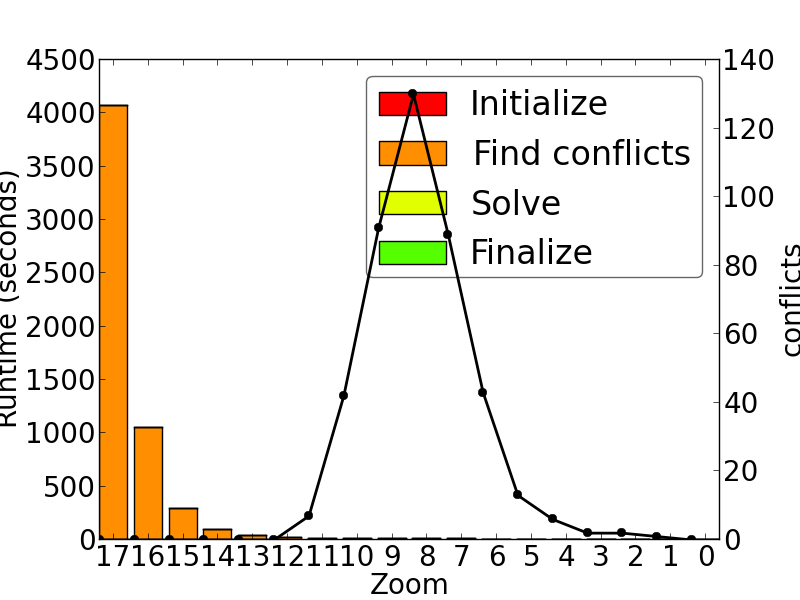
\includegraphics[width=1.0\linewidth]{./figs/prelim_lin_30k_uswaterway_heuristic_A.png}}
    \centerline{(a) LPGA + Visibility}
  \end{minipage} \hfill
  \begin{minipage}{0.329\linewidth}
    \centerline{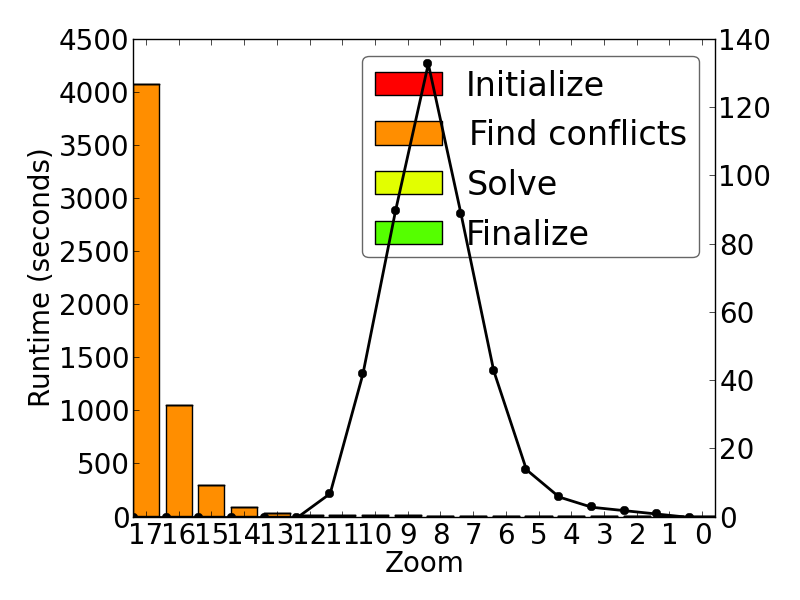
\includegraphics[width=1.0\linewidth]{./figs/prelim_lin_30k_uswaterway_lp_A.png}}
    \centerline{(b) SGA + Visibility}
  \end{minipage} \hfill
  \begin{minipage}{0.329\linewidth}
    \centerline{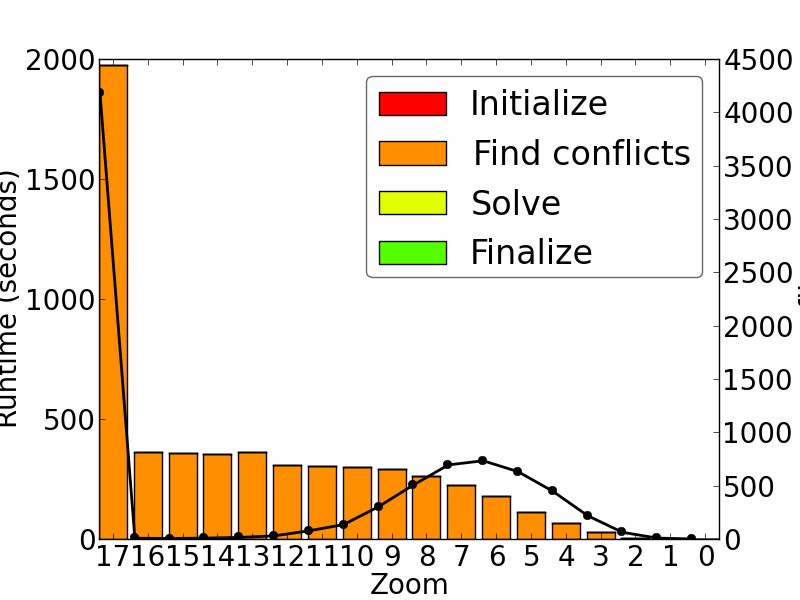
\includegraphics[width=1.0\linewidth]{./figs/prelim_lin_30k_uswaterway_lp_B.png}}
    \centerline{(c) Rivers: LPGA + Proximity}
  \end{minipage}
  \vspace{-0ex}
  \caption{Performance breakdown by zoom level, Rivers dataset (4K records). The black line indicates number of conflicts} \label{fig:performance:complex}
  \vspace{-2ex}
\end{figure*}


\minisec{Scalability}

In Figure~\ref{fig:scalability} we show scalability results for complex shape data. Here the scalability depends more on the choice of constraint than the choice of solver. The proximity constraint scales much worse than the visibility constraint. This is because the running time of the distance test used in the proximity constraint is proportional to the product of point counts in the two geometric shapes used in each comparison. Evaluating the visibility depends on the number of tiles that each shape intersects, which depends more on the length or area of each shape. 

While constraints matter more to scalability for complex shapes, the SGA solver scales better than LPGA, which was also the case for our point data.


% !TEX root = ./cvl.tex
\section{Related work}
\label{sec:related}
\marcos{One should make sure to include the items below.}

Basic reference set:

\begin{itemize}

\item Fusion Tables~\cite{sarma2012fusiontables}. 
% zoom consistency, adjacency, visibility; not general constraints. // different types of objectives, but no declarative interface and integration with standard database technology.

\item Summary and most important references from cartographic generalization survey.

\item Reverse data management vision~\cite{meliou2011reverse}

\end{itemize}

Additional references:

\begin{itemize}

\item In-database processing: briefly repeat argument with Pathfinder and Ferry (As we mentioned earlier,...). Increasingly, relational are incorporating whole programming language interpreters and support for spatial data structures~\cite{Blakeley2008:DotNET}. Then also cite MADLib work~\cite{hellerstein12madlib} as well as Ordonez~\cite{ordonez10udf}. But: direct SQL and not higher-level DSL leveraging SQL + analytics / statistics and not spatial.  

\item Say something about how you actually serve the map after it is built with our framework (e.g., the usual references in linearization)~\cite{hilbert1891ueber}.

\item ...

\marcos{Still performing scan of recent literature, just in case.}

\item if it fits, reverse / symbolic query processing.

\end{itemize}

\martin{We should mention that the dynamic greedy algorithm would have improved the running time compared to the LP-based greedy algorithm, while achieving good quality~\cite{rajagopalan1998primal}.}


% !TEX root = ./cvl.tex
\section{Acknowledgements}
This project has been funded by Grontmij, the Danish Geodata Agency and the Ministry of Innovation in Denmark. We would like to thank employees and management at Grontmij and the Danish Geodata Agency for great discussions about the ideas presented in this work. We would also like to thank Amazon for providing an AWS in education grant which we used to implement our experimental setup.

% !TEX root = ./cvl.tex
\section{Conclusion}


% The following two commands are all you need in the
% initial runs of your .tex file to
% produce the bibliography for the citations in your paper.
\bibliographystyle{abbrv}
\bibliography{cvl}  % gvl.bib is the name of the Bibliography in this case
% You must have a proper ".bib" file
%  and remember to run:
% latex bibtex latex latex
% to resolve all references


\end{document}
